\chapter{Trigonometric Identities}

\section{The Unit Circle}
First, there are some values of $\sin{\theta}$ and $\cos{\theta}$ that will be 
useful to know off the top of your head. The Unit Circle will help you in this 
memorization process (see figure \ref{fig:unit_cicle_blank}). When a circle of 
radius 1 is centered at the origin, the Cartesian coordinates of any point on 
the circle correspond to the values of cosine and sine of the angle above 
the horizontal (how far you've rotated from the positive $x$-axis). 

\begin{figure}[htbp]
    \centering
    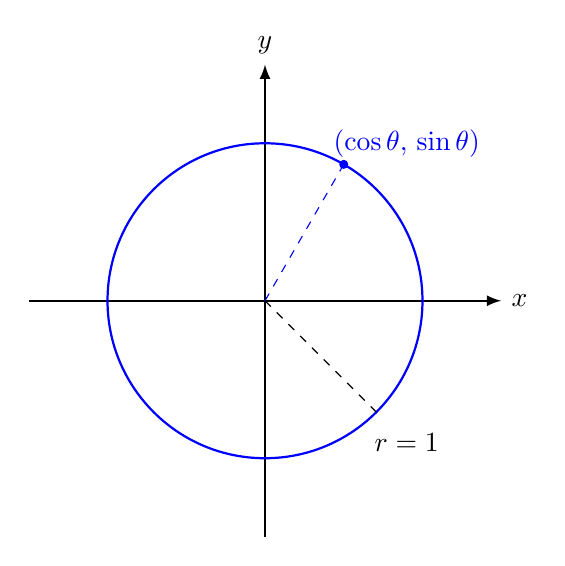
\begin{tikzpicture}
        \draw[-latex, thick] (-3, 0) -- (3, 0) node[right] {$x$};
        \draw[-latex, thick] (0, -3) -- (0, 3) node[above] {$y$};
        \draw[blue, thick] (0,0) circle (2);
        \draw[blue, dashed] (0,0) -- (1, 1.732);
        \draw[blue, fill=blue] (1, 1.732) circle (0.05);
        \node[blue] at (1.8, 2) {$(\cos{\theta}$, $\sin{\theta})$};
        \draw[black, dashed] (0,0) -- (1.414, -1.414);
        \node[] at (1.8, -1.8) {$r=1$};
    \end{tikzpicture}
    \caption{The Unit Circle is a circle with radius 1 centered at the origin}
    \label{fig:unit_cicle_blank}
\end{figure}

Let's take a closer look at a triangle in the first quadrant to see why this 
is true. Imagine some point on the circle, $(x_o, y_o)$. Drawing a line from 
that point back to the origin creates an angle $\theta$ between the imaginary 
line and the positive $x$-axis (see figure \ref{fig:unit_cicle_zoom}). 
Extending an imaginary vertical down to $(x_o, 0)$ and then an imaginary 
horizontal from $(x_o, 0)$ to the origin creates a right triangle. What can we 
say about the legs of the triangle?

\begin{figure}[htbp]
    \centering
    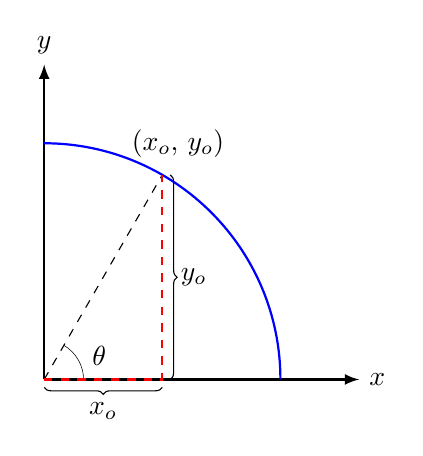
\begin{tikzpicture}
        \draw[-latex, thick] (0, 0) -- (4, 0) node[right] {$x$};
        \draw[-latex, thick] (0, 0) -- (0, 4) node[above] {$y$};
        \draw[blue, thick] (3,0) arc [start angle = 0, end angle = 90, 
        x radius = 3, y radius = 3];
        \draw[black, dashed] (0,0) -- (1.5, 2.598);
        \draw[black, very thin] (0.5, 0) arc [start angle = 0, end angle = 60, 
        x radius = 0.5, y radius = 0.5];
        \node[] at (1.7, 3) {$(x_o$, $y_o)$};
        \node[] at (0.7, 0.3) {$\theta$};
        \draw[red, thick, dashed] (0,0) -- (1.5, 0) -- (1.5, 2.598);
        \draw[decorate, decoration=brace] (1.6, 2.598) -- (1.6, 0) node[midway, 
        xshift = 0.3cm] {$y_o$};
        \draw[decorate, decoration=brace] (1.5, -0.1) -- (0, -0.1) node[midway, 
        yshift = -0.3cm] {$x_o$};
    \end{tikzpicture}
    \caption{Drawing a line from any point on the circle to the origin creates 
    an angle with the horizontal}
    \label{fig:unit_cicle_zoom}
\end{figure}

Recall SOH-CAH-TOA from a previous chapter. This acronym tells us that, for a 
right triangle, the sine of an angle is given by the ratio of the length of the
leg opposite the angle to the hypotenuse. Then, in our case, $\sin{\theta} = 
\frac{y_o}{1} = y_o$. [Remember: we are dealing with the Unit Circle, which has
a radius of one. Examining figure \ref{fig:unit_cicle_zoom} shows you that the 
hypotenuse of the imaginary triangle is the same as the circle's radius.] This 
means that the $y$-coordinate of any point on the Unit Circle is the sine of 
the angle of rotation from the horizontal. 

\begin{Exercise}[label = sine]
In a similar manner as we did with $\sin{\theta}$ above, prove the 
$x$-coordinate of any point on the unit circle is equal to $\cos{\theta}$, 
where $\theta$ is the angle of rotation from the horizontal. 
\vspace{20mm}
\end{Exercise}

\begin{Answer}[ref = sine]
We know that for a right triangle, $\cos{\theta} = \frac{\text{adjacent leg}}{
\text{hypotenuse}}$. For a right triangle inscribed in the Unit Circle, the 
adjacent leg is parallel to the $x$-axis and has the same length as the 
$x$-value of the coordinate point on the circle. Additionally, the length of 
the hypotenuse is 1. Therefore, $\cos{\theta} = \frac{x_o}{1} = x_o$. 
\end{Answer}

\begin{Exercise}[label = unit_circle1]
[fixme fill in sine and cosine for 0, pi/2, pi, 3pi/2]
\end{Exercise}

\subsection{Exact Values of Key Angles}
We will examine two triangles: a 30-60-90 triangle and a 45-45-90 triangle. 
First, the 30-60-90. As shown in figure \ref{fig:306090}, you can get a 
30-60-90 triangle with hypotenuse 1 by dividing an equilateral triangle in 
half. We will label the horizontal leg of the 30-60-90 triangle A and the 
vertical leg B. 

\begin{figure}[htbp]
    \centering
    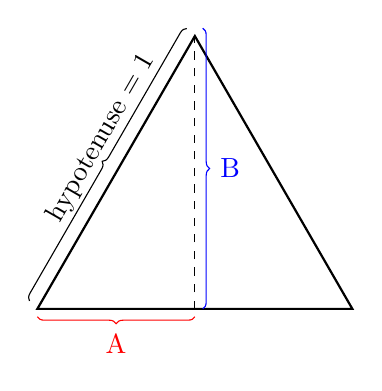
\begin{tikzpicture}
        \draw[thick] (-2, 0) -- (2, 0) -- (0, 3.464) -- cycle;
        \draw[dashed] (0,0) -- (0,3.464);
        \draw[decorate, decoration=brace] (-2.1, 0.1) -- (-0.1, 3.564)  node[
        midway, rotate=60, xshift = 0.25cm, yshift = 0.25cm] {hypotenuse = 1};
        \draw[red, decorate, decoration=brace] (0,-0.1) -- (-2, -0.1) node[
        midway, yshift = -0.35cm] {A};
        \draw[blue, decorate, decoration = brace] (0.1, 3.564) -- (0.1, 0)  
        node[midway, xshift=0.35cm] {B};
    \end{tikzpicture}
    \caption{A 30-60-90 triangle is made by vertically bisecting an equilateral
    triangle}
    \label{fig:306090}
\end{figure}

From the figure, we see that the length of A is half that of the hypotenuse, 
which in this case is $\frac{1}{2}$. This means the $\cos{60^{\circ}} = \cos{
\frac{\pi}{3}} = \frac{1}{2}$. To find the length of side B, we can use the 
Pythagorean theorem:
$$B^2 = C^2 - A^2\text{, where C is the hypotenuse}$$
$$B^2 = 1^2 - \left( \frac{1}{2} \right)^2$$
$$B^2 = \frac{3}{4}$$
$$B = \frac{\sqrt{3}}{2}$$

And therefore, $\sin{60^{\circ}} = \sin{\frac{\pi}{3}} = \frac{\sqrt{3}}{2}$. 

\begin{Exercise}[label=unit_circle2]
Use symmetry to complete the blank unit circle below. (Hint: we just shown 
that the $(x,y)$ coordinate for $\frac{\pi}{3}$ is $(1/2, \sqrt{3}/2)$). 

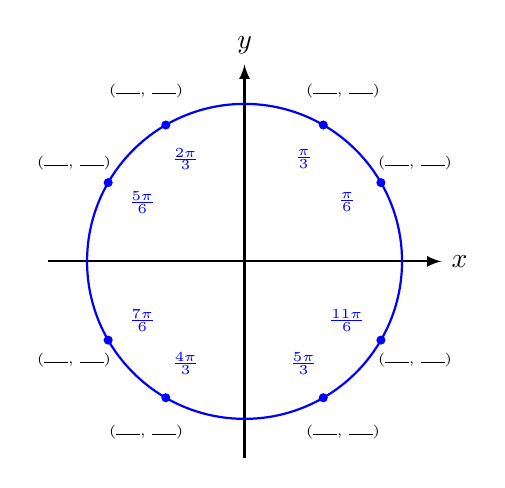
\begin{tikzpicture}
        \draw[thick, -latex] (-2.5, 0) -- (2.5, 0) node[right] {$x$};
        \draw[thick, -latex] (0, -2.5) -- (0, 2.5) node[above] {$y$};
        \draw[blue, thick] (0,0) circle (2);
        \foreach \x/\y/\t in {1.732/1/$\frac{\pi}{6}$, 1/1.732/$\frac{\pi}{3}$,
        -1/1.732/$\frac{2\pi}{3}$, -1.732/1/$\frac{5\pi}{6}$, 
        -1.732/-1/$\frac{7\pi}{6}$, -1/-1.732/$\frac{4\pi}{3}$, 
        1/-1.732/$\frac{5\pi}{3}$, 1.732/-1/$\frac{11\pi}{6}$} {
        \draw[blue, fill=blue] (\x, \y) circle (0.05);
        \node[blue, font=\tiny] at (0.75*\x, 0.75*\y) {\t};
        \node[font=\tiny] at (1.25*\x, 1.25*\y) {(\rule{0.3cm}{0.15mm}, \rule{
        0.3cm}{0.15mm})};
        }
    \end{tikzpicture}
\end{Exercise}

\begin{Answer}[ref = unit_circle2]
[fixme answer to exercise]
\end{Answer}

\section{Sum and Difference Formulas}
Consider 4 points on the unit circle: $B$ at $(1, 0)$, $Q$ at some angle 
$\beta$, $P$ at some angle $\alpha$, and $A$ at angle $\alpha - \beta$ (see 
figure \ref{fig:difference}). 

\begin{figure}[htbp]
    \centering
    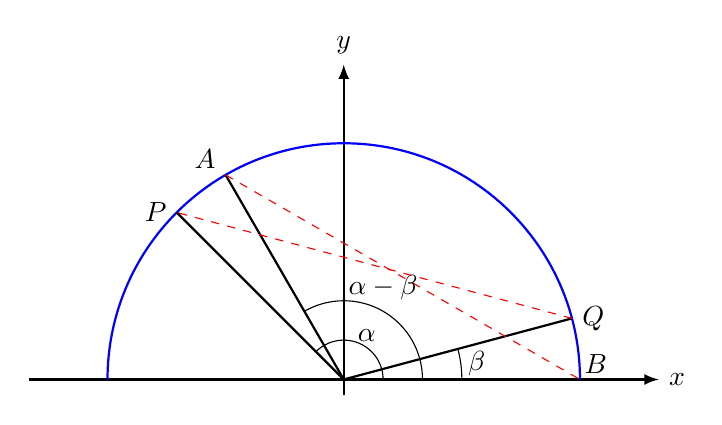
\begin{tikzpicture}
        \draw[-latex, thick] (-4, 0) -- (4, 0) node[right] {$x$};
        \draw[-latex, thick] (0, -0.2) -- (0, 4) node[above] {$y$};
        \draw[blue, thick] (3,0) arc [start angle = 0, end angle = 180, 
        x radius = 3, y radius = 3];
        \draw[thick] (0,0) -- (2.898, 0.776) node[right] {$Q$};
        \draw[thick] (0,0) -- (-1.5, 2.598) node[left, yshift = 0.2cm] {$A$};
        \draw[red, dashed] (2.898, 0.776) -- (-2.121, 2.121);
        \draw[thick] (0,0) -- (-2.121, 2.121) node[left] {$P$};
        \node[] at (3.2, 0.2) {$B$};
        \draw[red, dashed] (-1.5, 2.598) -- (3, 0);
        \draw[thin] (1.5, 0) arc [start angle = 0, end angle = 15, x radius = 
        1.5, y radius = 1.5] node[midway, xshift = 0.2cm] {$\beta$};
        \draw[thin] (1, 0) arc [start angle = 0, end angle = 120, x radius = 1,
        y radius = 1] node[midway, yshift = 0.3cm] {$\alpha - \beta$};
        \draw[thin] (0.5, 0) arc[start angle = 0, end angle = 135, x radius = 
        0.5, y radius = 0.5] node[midway, xshift = 0.1cm, yshift = 0.1cm] 
        {$\alpha$};
    \end{tikzpicture}
    \caption{$\overline{AB} = \overline{PQ}$}
    \label{fig:difference}
\end{figure}

Then the distance from $P$ to $Q$ is the same as the distance from $A$ to $B$, 
since $\Delta POQ$ is a rotation of $\Delta AOB$. Because this is a Unit 
Circle, $P = (\cos{\alpha}, \sin{\alpha})$, $Q = (\cos{\beta}, \sin{\beta})$, 
and $A = (\cos{\alpha - \beta}, \sin{\alpha - \beta})$. Let us use the distance
formula to find the length of $\overline{PQ}$:
$$\overline{PQ} = \sqrt{\left(\cos{\alpha} - \cos{\beta} \right)^2 + \left( 
\sin{\alpha} - \sin{\beta} \right)^2} =$$
$$\sqrt{\cos^2{\alpha} - 2\cos{\alpha}\cos{\beta} + \cos^2{\beta} + \sin^2{
\alpha} - 2\sin{\alpha}\sin{\beta} + \sin^2{\beta}} = $$
$$\sqrt{\left( \cos^2{\alpha} + \sin^2{\alpha} \right) + \left( \cos^2{\beta} 
+ \sin^2{\beta} \right) - 2\cos{\alpha}\cos{\beta} - 2\sin{\alpha}\sin{\beta}}
$$

Recall that for any angle, $\theta$, $\sin^2{\theta} + \cos^2{\theta} = 1$. 
Substituting this identity, we see that:
$$\overline{PQ} = \sqrt{1 + 1 -2\sin{\alpha}\sin{\beta} - 2\cos{\alpha}\cos{
\beta}} = \sqrt{2 - 2\sin{\alpha}\sin{\beta} - 2\cos{\alpha}\cos{\beta}}$$

Let's leave this simplified equation for $\overline{PQ}$ alone for the moment 
and similarly find $\overline{AB}$:
$$\overline{AB} = \sqrt{\left[ \cos{\left( \alpha - \beta \right)} - 1 \right]^
2 + \left[ \sin{\left( \alpha - \beta \right)} - 0 \right]^2} = $$
$$\sqrt{\cos^2{ \left( \alpha - \beta \right)} - 2\cos{ \left( \alpha - \beta 
\right)} + 1 + \sin^2{ \left( \alpha - \beta \right)}} = $$
$$\sqrt{\cos^2{ \left( \alpha - \beta \right)} + \sin^2{ \left( \alpha - \beta 
\right)} + 1 - 2\cos{ \left( \alpha - \beta \right)}} $$
$$= \sqrt{2 - 2\cos{ \left( \alpha - \beta \right)}} = \overline{AB}$$

Recall that we've established $\overline{AB} = \overline{PQ}$. Then we can set 
the statements equal to each other:
$$ \sqrt{2 - 2\sin{\alpha}\sin{\beta} - 2\cos{\alpha}\cos{\beta}} = \sqrt{2 - 2
\cos{ \left( \alpha - \beta \right)}}$$

Squaring both sides and subtracting 2, we find:
$$-2\sin{\alpha}\sin{\beta} - 2\cos{\alpha}\cos{\beta} = -2\cos{\left( \alpha -
\beta \right)}$$

Finally, we can divide both sides by negative 2 and we get the difference of 
angles formula for cosine:
$$\cos{ \left( \alpha - \beta \right)} = \cos{\alpha}\cos{\beta} + \sin{\alpha}
\sin{\beta}$$

There are similar formulas for the sine and cosine of the sum of two angles and
for the sine of the difference of two angles, which we won't derive here. 

\begin{mdframed}[style=important, frametitle={Sum and Difference Formulas}]
$$\cos{ \left( \alpha + \beta \right)} = \cos{\alpha}\cos{\beta} - \sin{\alpha}\sin{\beta}$$
$$\cos{ \left( \alpha - \beta \right)} = \cos{\alpha}\cos{\beta} + \sin{\alpha}\sin{\beta}$$
$$\sin{ \left( \alpha + \beta \right)} = \sin{\alpha}\cos{\beta} + \cos{\alpha}\sin{\beta}$$
$$\sin{ \left( \alpha - \beta \right)} = \sin{\alpha}\cos{\beta} - \cos{\alpha}\sin{\beta}$$
\end{mdframed}

\begin{Exercise}[label = sum_diff]
Without a calculator, find the exact value requested:
\begin{enumerate}
\item $\sin{\frac{\pi}{12}}$
\item $\cos{\frac{7\pi}{12}}$
\item $\tan{\frac{13\pi}{12}}$ (hint: $\tan{\theta} = \sin{\theta}/\cos{\theta}$)
\end{enumerate}
\end{Exercise}

\section{Double and Half Angle Formulas}